\chapter{Resultados}
\label{ch:resultados}

En el capitulo {\ref{ch:metodos} presentamos la t\'ecnica de 
\textit{bootstraping}; el m\'etodo de Moreno-Dominguez para agrupar
tractogramas junto con algunas de sus falencias te\'oricas y como
solucionarlas usando la funci\'on \textit{logit}. En la secci\'on 
\ref{ch:nuestro}, presentamos nuestro m\'etodo para parcelar la corteza en
su totalidad. En las siguientes secciones mostramos primero los resultados
obtenidos al estudiar la estabilidad de los tractogramas; luego parcelamos
el \'area de Broca con ambos m\'etodos y finalmente parcelamos el
hemisferio derecho usando tambi\'en ambos m\'etodos. Todos los estudios se
realizaron sobre una misma mujer diestra de entre 23 y 26 a\~nos. Sus datos
fueron descargados de la base de datos \textit{Human Connectome Project}
\cite{VanEssen2012}.


\section{Estabilidad tractogramas}

Las Figuras \ref{fig:m1}, \ref{fig:m2} y \ref{fig:m3} muestran, para tres semillas
distintas, cinco cortes axiales del tractograma que se consigue al utilizar quince
mil part\'iculas.\\

Las Figuras \ref{fig:s1}, \ref{fig:s2} y \ref{fig:s3} muestran la varianza de 
cada voxel dentro de un mismo corte axial. La varianza se calcul\'o generando
mil tractogramas desde distinto n\'umero de streamlines. \\

La Figura \ref{fig:mv} muestra la media y varianza de los voxels $A$, $B$ y $C$
marcados en las Figuras \ref{fig:s1}, \ref{fig:s2} y \ref{fig:s3}. Estos voxels
fueron los que mayor varianza presentaron al generar tractogramas con dos mil
\textit{streamlines}.


\begin{figure}[h!]
   \centering
    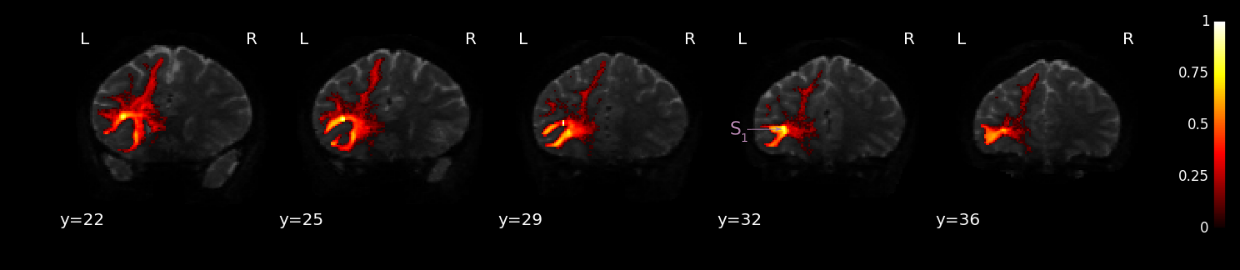
\includegraphics[width=\textwidth]{img/m1.png}
    \caption{Tractograma para la semilla $S1$ utilizando toda la muestra.}
    \label{fig:m1}
\end{figure}

\begin{figure}[h!]
   \centering
    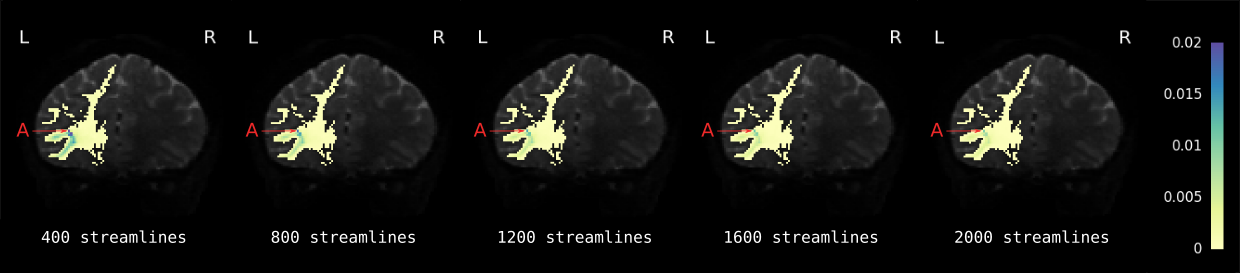
\includegraphics[width=\textwidth]{img/s1.png}
    \caption{Desviaci\'on Estandar respecto a la semilla $S1$. Mismo corte axial
             variando el tama\~no de las submuestras.}
    \label{fig:s1}
\end{figure}

\begin{figure}[h!]
   \centering
    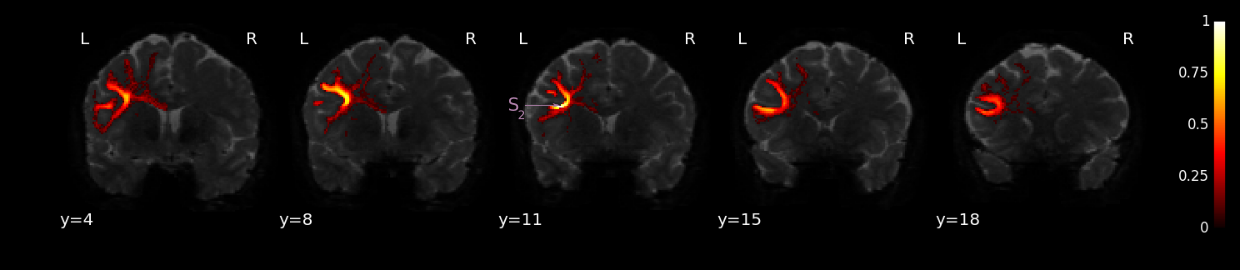
\includegraphics[width=\textwidth]{img/m2.png}
    \caption{Tractograma para la semilla $S2$ utilizando toda la muestra.}
    \label{fig:m2}
\end{figure}

\begin{figure}[h!]
   \centering
    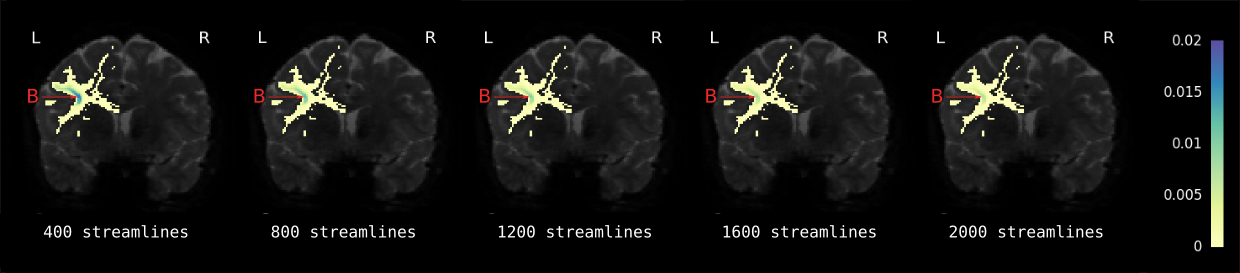
\includegraphics[width=\textwidth]{img/s2.png}
    \caption{Desviaci\'on Estandar respecto a la semilla $S2$. Mismo corte axial
             variando el tama\~no de las submuestras.}
    \label{fig:s2}
\end{figure}

\begin{figure}[h!]
   \centering
    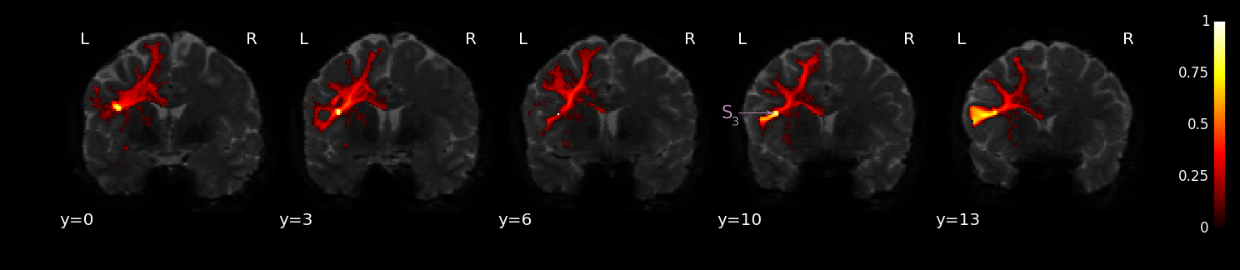
\includegraphics[width=\textwidth]{img/m3.png}
    \caption{Tractograma para la semilla $S3$ utilizando toda la muestra}
    \label{fig:m3}
\end{figure}

\begin{figure}[h!]
   \centering
    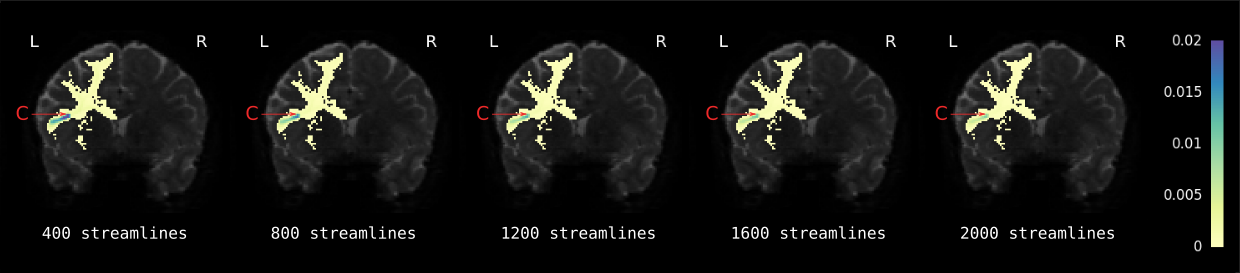
\includegraphics[width=\textwidth]{img/s3.png}
    \caption{Desviaci\'on Estandar respecto a la semilla $S3$. Mismo corte axial
             variando el tama\~no de las submuestras.}
    \label{fig:s3}
\end{figure}

\begin{figure}[h!]
   \centering
    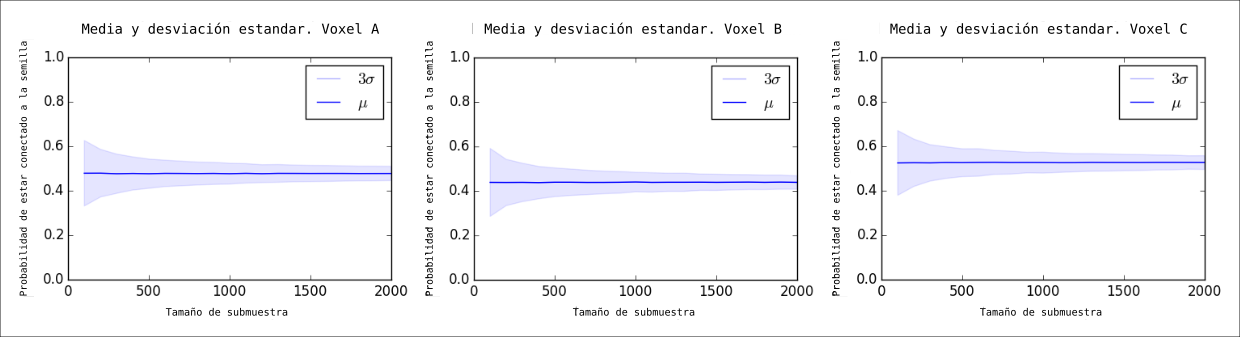
\includegraphics[width=\textwidth]{img/med_var_all.png}
    \caption{Media y desviaci\'on estandar de los voxels con mayor varianza.}
    \label{fig:mv}
\end{figure}


\section{Parcelando el \'Area de Broca}

\subsection{Distancia coseno con centroide}

Las siguientes Figuras muestran los resultados obtenidos al parcelar el \'Area
de Broca utilizando el m\'etodo de Moreno-Dominguez.

\begin{figure}[h!]
                                                                                                                        
\begin{minipage}[b]{\textwidth}
    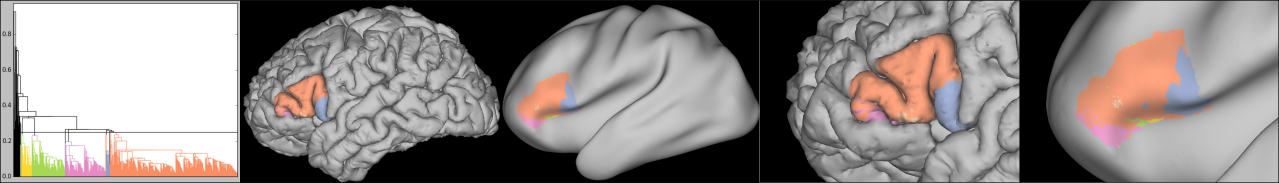
\includegraphics[width=\textwidth]{img/broca/moreno_0.png}
    \caption{M\'etodo Moreno sin preprocesamiento}

\end{minipage} ~
                                                                                                                       
\begin{minipage}[b]{\textwidth}
    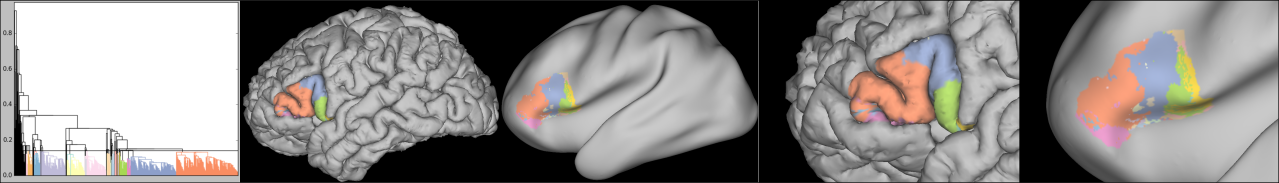
\includegraphics[width=\textwidth]{img/broca/moreno_0_deep.png}
    \caption{M\'etodo Moreno sin preprocesamiento, mayor profundidad en el 
            dendrograma}

\end{minipage} ~

\begin{minipage}[b]{\textwidth}
    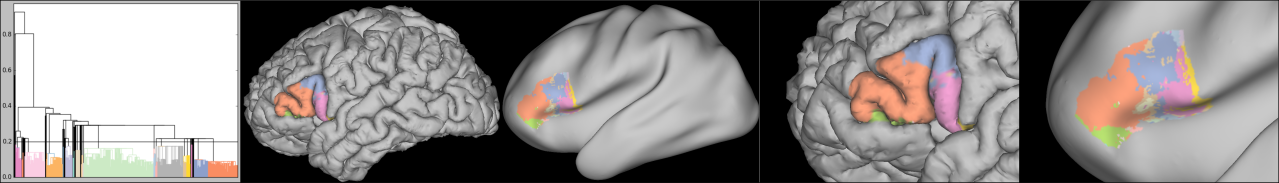
\includegraphics[width=\textwidth]{img/broca/moreno_400.png}
    \caption{M\'etodo Moreno, cuatrocientos pasos de preprocesamiento}

\end{minipage} ~

\begin{minipage}[b]{\textwidth}
    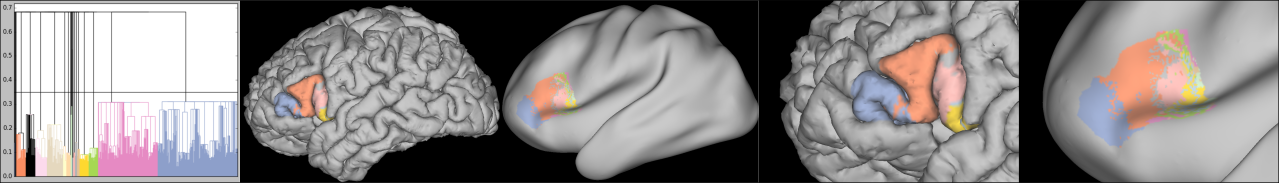
\includegraphics[width=\textwidth]{img/broca/moreno_750.png}
    \caption{M\'etodo Moreno, setecientos pasos de preprocesamiento}

\end{minipage} ~

\end{figure} 


\subsection{Utilizando LogOdds}

Las siguientes Figuras muestran los resultados obtenidos al parcelar el \'Area
de Broca utilizando el m\'etodo de Moreno-Dominguez. El threshold utilizado fue
de $0.25$. \textbf{Los resultados obtenidos luego de normalizar los vectores 
fueron tan malos que no vale la pena incluirlos}.

\begin{figure}[h!]
                                                                                                                        
\begin{minipage}[b]{\textwidth}
    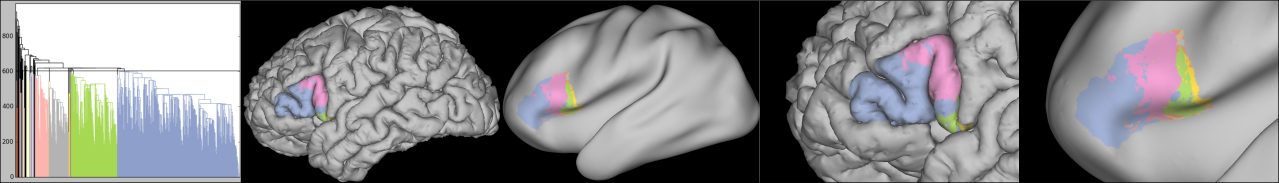
\includegraphics[width=\textwidth]{img/broca/logit_0.png}
    \caption{M\'etodo Logit sin preprocesamiento}
    \label{fig:dmri}
\end{minipage} ~
                                                                                                                        
\begin{minipage}[b]{\textwidth}
    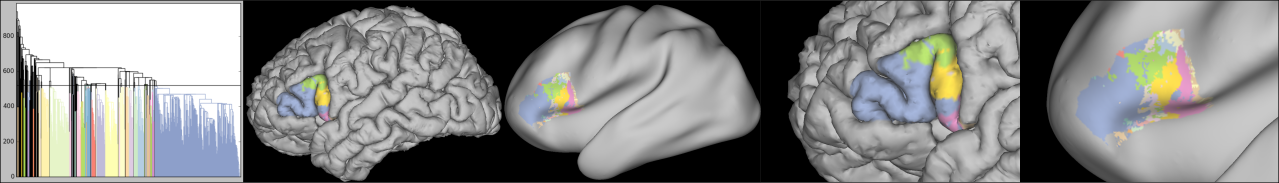
\includegraphics[width=\textwidth]{img/broca/logit_0_deep.png}
    \caption{M\'etodo Logit sin preprocesamiento, mayor profundidad en el 
            dendrograma}

\end{minipage} ~

\begin{minipage}[b]{\textwidth}
    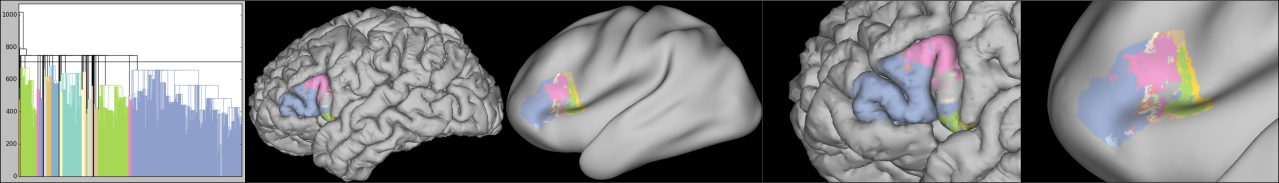
\includegraphics[width=\textwidth]{img/broca/logit_400.png}
    \caption{M\'etodo Logit, cuatrocientos pasos de preprocesamiento}

\end{minipage} ~

\begin{minipage}[b]{\textwidth}
    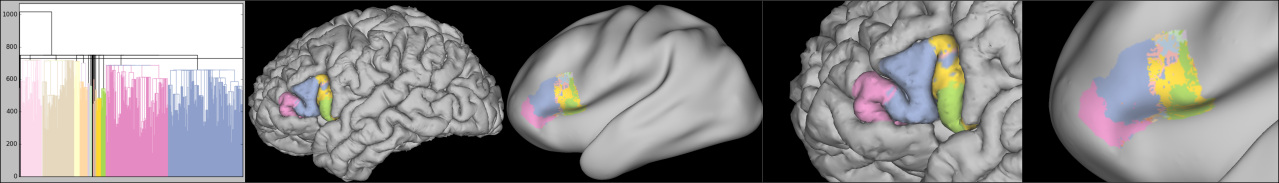
\includegraphics[width=\textwidth]{img/broca/logit_750.png}
    \caption{M\'etodo Logit, setecientos pasos de preprocesamiento}

\end{minipage} ~

\end{figure}


\subsection{Lado a lado}


\begin{figure}[h]

\begin{minipage}[h]{\textwidth}
    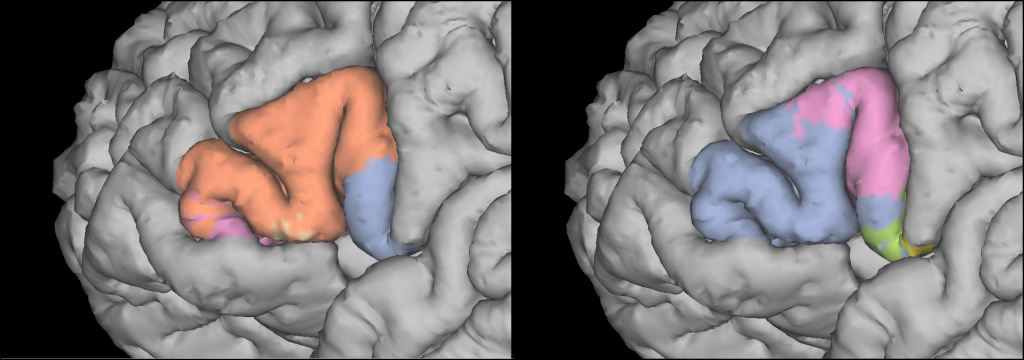
\includegraphics[width=\textwidth]{img/broca/vs_0.png}
    \caption{M\'etodo Moreno (izquierda) y Logit (derecha) sin preprocesamiento}
\end{minipage} ~

\end{figure}

\begin{figure}[h]                  

\begin{minipage}[h]{\textwidth}
    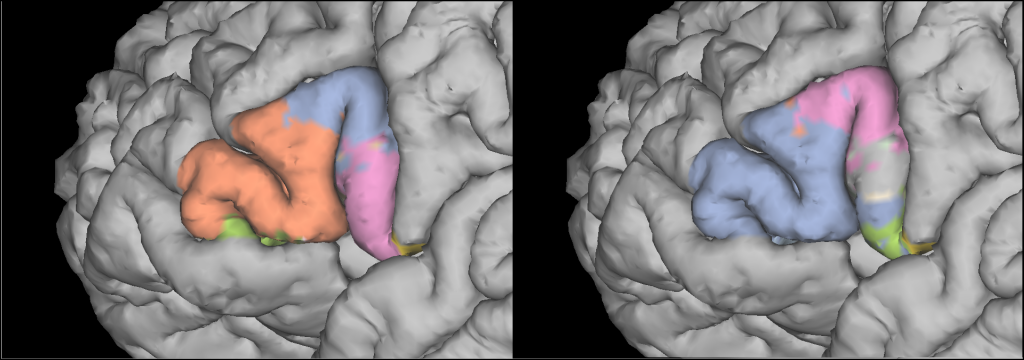
\includegraphics[width=\textwidth]{img/broca/vs_400.png}
    \caption{M\'etodo Moreno (izquierda) y Logit (derecha). Cuatrocientos pasos de preprocesamiento}
\end{minipage} ~

\end{figure}

\begin{figure}[h]

\begin{minipage}[h]{\textwidth}
    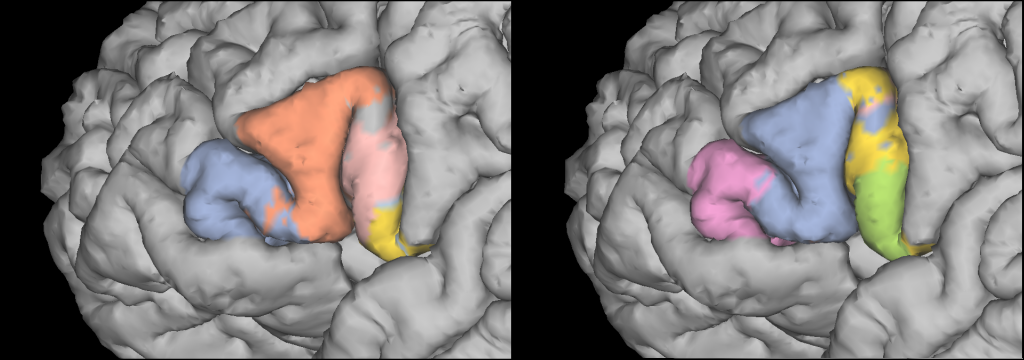
\includegraphics[width=\textwidth]{img/broca/vs_700.png}
    \caption{M\'etodo Moreno (izquierda) y Logit (derecha). Setecientos pasos de preprocesamiento}

\end{minipage} ~

\end{figure}
 


\section{Parcelando la corteza}

\subsection{Utilizando LogOdds}

\begin{figure}[h!]
                                                                                                                        
\begin{minipage}[b]{\textwidth}
    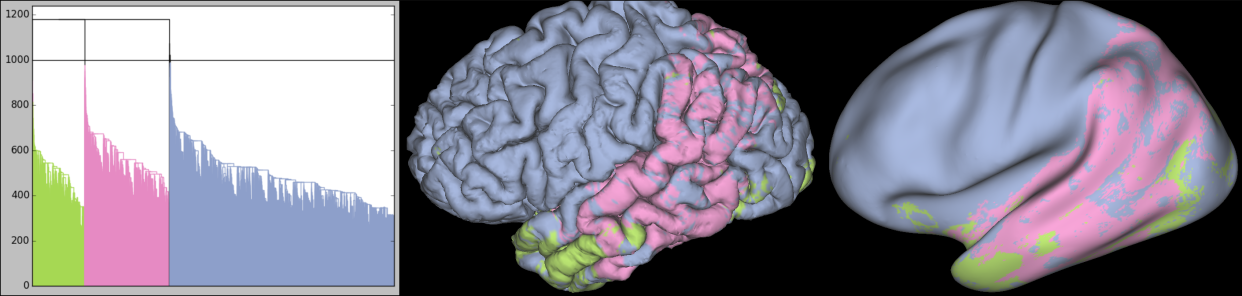
\includegraphics[width=\textwidth]{img/all_brain/logit_0.png}
    \caption{M\'etodo Logit sin preprocesamiento}
    \label{fig:dmri}
\end{minipage} ~
                                                                                                                        
\begin{minipage}[b]{\textwidth}
    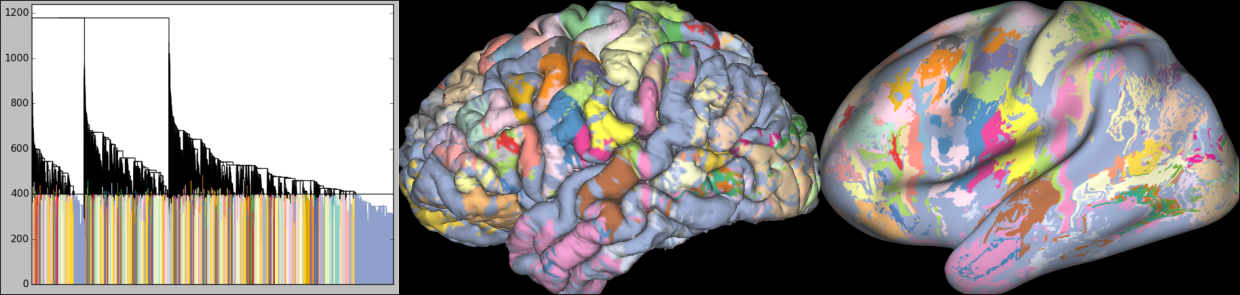
\includegraphics[width=\textwidth]{img/all_brain/logit_0_deep.png}
    \caption{M\'etodo Logit sin preprocesamiento, mayor profundidad en el 
            dendrograma}

\end{minipage} ~

\begin{minipage}[b]{\textwidth}
    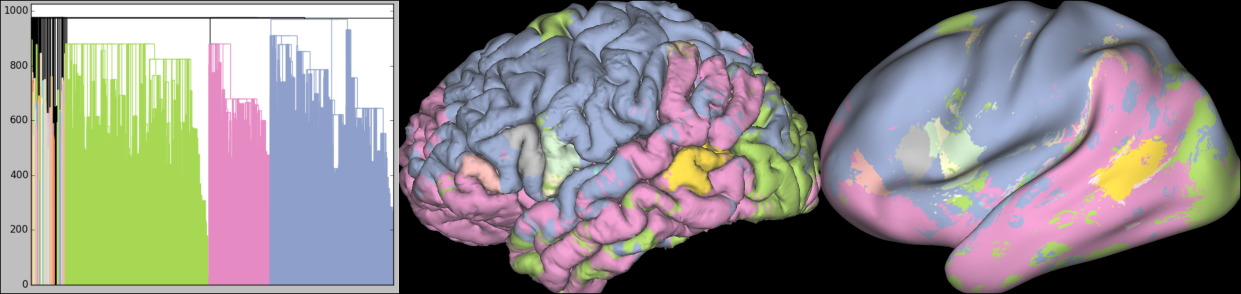
\includegraphics[width=\textwidth]{img/all_brain/logit_20000.png}
    \caption{M\'etodo Logit, veinte mil pasos de preprocesamiento}

\end{minipage} ~

\begin{minipage}[b]{\textwidth}
    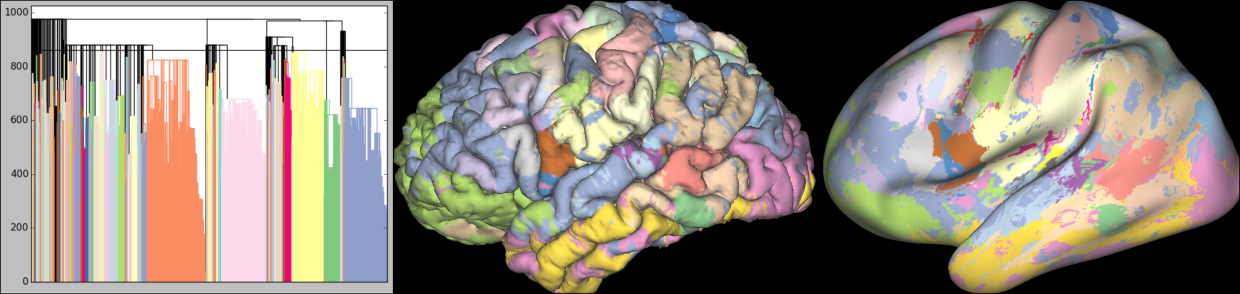
\includegraphics[width=\textwidth]{img/all_brain/logit_20000_deep0.png}
    \caption{M\'etodo Logit, veinte mil pasos de preprocesamiento, mayor 
             profundidad}
\end{minipage} ~

\begin{minipage}[b]{\textwidth}
    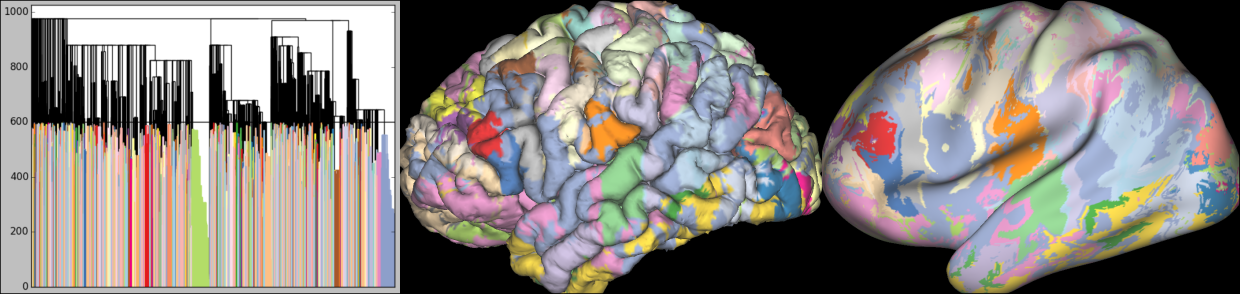
\includegraphics[width=\textwidth]{img/all_brain/logit_20000_deep1.png}
    \caption{M\'etodo Logit, veinte mil pasos de preprocesamiento, mayor 
             profundidad}
\end{minipage} ~


\end{figure}

